% =====================================================================
%  CiteGuard: LLM-Based Fake Citation Detection and Verification System
%  ILLM Final Project Presentation -- Beamer (Madrid), 16:9
%  Compile with: tectonic presentation.tex   (or pdflatex, run twice)
%  Figures are read from ./assets/
% =====================================================================
\PassOptionsToPackage{table}{xcolor}
\documentclass[aspectratio=169,10pt]{beamer}

\usepackage{amsmath,amssymb}
\usepackage{graphicx}
\usepackage{booktabs}
\usepackage{multirow}
\usepackage{array}
\usepackage{tikz}
\usetikzlibrary{shapes.geometric,arrows.meta,positioning,fit,backgrounds}
\usepackage{hyperref}

\usetheme{Madrid}
\usecolortheme{default}

\definecolor{accentblue}{RGB}{0,84,166}
\definecolor{lightblue}{RGB}{220,235,250}
\definecolor{darkblue}{RGB}{0,50,120}
\definecolor{goodgreen}{RGB}{214,240,214}
\definecolor{warnorange}{RGB}{255,232,204}
\definecolor{badred}{RGB}{192,57,43}
\definecolor{llmpurple}{RGB}{237,233,254}
\definecolor{llmborder}{RGB}{109,40,217}

\setbeamercolor{structure}{fg=accentblue}
\setbeamercolor{palette primary}{bg=accentblue,fg=white}
\setbeamercolor{palette secondary}{bg=darkblue,fg=white}
\setbeamercolor{palette tertiary}{bg=darkblue,fg=white}
\setbeamercolor{palette quaternary}{bg=darkblue,fg=white}
\setbeamercolor{frametitle}{bg=accentblue,fg=white}
\setbeamercolor{title}{bg=accentblue,fg=white}
\setbeamercolor{block title}{bg=accentblue,fg=white}
\setbeamercolor{block body}{bg=lightblue,fg=black}
\setbeamercolor{block title alerted}{bg=darkblue,fg=white}
\setbeamercolor{block body alerted}{bg=lightblue,fg=black}
\setbeamercolor{block title example}{bg=darkblue,fg=white}
\setbeamercolor{block body example}{bg=lightblue,fg=black}
\setbeamercolor{section in toc}{fg=darkblue}
\setbeamercolor{alerted text}{fg=accentblue}

\setbeamertemplate{itemize items}[circle]
\setbeamertemplate{enumerate items}[circle]
\setbeamertemplate{sections/subsections in toc}[circle]
\setbeamertemplate{navigation symbols}{}
\setbeamertemplate{blocks}[rounded][shadow=false]
\setbeamerfont{caption}{size=\scriptsize}

\setbeamertemplate{footline}{%
  \leavevmode%
  \hbox{%
    \begin{beamercolorbox}[wd=.333\paperwidth,ht=2.4ex,dp=1ex,center]{palette primary}%
      \usebeamerfont{author in head/foot}\insertshortauthor
    \end{beamercolorbox}%
    \begin{beamercolorbox}[wd=.334\paperwidth,ht=2.4ex,dp=1ex,center]{palette secondary}%
      \usebeamerfont{title in head/foot}\insertshorttitle
    \end{beamercolorbox}%
    \begin{beamercolorbox}[wd=.333\paperwidth,ht=2.4ex,dp=1ex,right]{palette primary}%
      \usebeamerfont{date in head/foot}\insertshortdate\hspace*{2em}%
      \insertframenumber{} / \inserttotalframenumber\hspace*{2ex}
    \end{beamercolorbox}}%
  \vskip0pt%
}

\setlength{\leftmargini}{1.2em}
\setlength{\leftmarginii}{1.2em}

\graphicspath{{assets/}}

\newcolumntype{P}[1]{>{\raggedright\arraybackslash}p{#1}}
\newcommand{\hl}[1]{\textcolor{accentblue}{\textbf{#1}}}
\newcommand{\bad}[1]{\textcolor{badred}{\textbf{#1}}}
\newcommand{\gc}[1]{\cellcolor{goodgreen}#1}
\newcommand{\na}{\textcolor{gray}{--}}

\tikzset{
  box/.style={draw=accentblue, fill=lightblue, rounded corners=3pt, thick,
              align=center, font=\scriptsize, minimum height=0.9cm, inner sep=4pt},
  dbox/.style={draw=darkblue, fill=accentblue, text=white, rounded corners=3pt,
              thick, align=center, font=\scriptsize\bfseries, minimum height=0.9cm, inner sep=4pt},
  lbox/.style={draw=llmborder, fill=llmpurple, rounded corners=3pt, thick,
              align=center, font=\scriptsize, minimum height=0.9cm, inner sep=4pt},
  arr/.style={-{Stealth[length=2.2mm]}, thick, darkblue},
  lbl/.style={font=\tiny, text=darkblue, align=center}
}

\title[CiteGuard: Fake Citation Detection]
{CiteGuard: LLM-Based Fake Citation Detection and Verification System}
\subtitle{Evidence decides whether a paper exists; the LLM explains, repairs and checks claims}
\author[Gandhi, Andhariya, Bateriwala, Dharodiya]
{Miten Gandhi (U23AI017) \and Harshil Andhariya (U23AI021) \and\\
 Vatsal Bateriwala (U23AI030) \and Aksh Dharodiya (U23AI031)}
\institute[SVNIT Surat]
{Department of Artificial Intelligence\\
Sardar Vallabhbhai National Institute of Technology, Surat\\[4pt]
\scriptsize Introduction to Large Language Models (ILLM) -- Final Project Presentation}
\date[\today]{\today}

\begin{document}

\begin{frame}[plain]
  \titlepage
\end{frame}

% =====================================================================
\section{Introduction}

\begin{frame}{Problem Statement}
  \begin{block}{Problem}
    \small Given a paper, a BibTeX file, a reference list or a chatbot's answer, decide for
    \hl{every citation} whether it refers to a real publication, whether its details are correct,
    \hl{explain why}, and propose a fix.
  \end{block}
  \vspace{2pt}
  \begin{columns}[T]
    \begin{column}{0.50\textwidth}
      \begin{alertblock}{A citation an LLM might write}
        \small
        Zhang, L., \& Kumar, R. (2021). \bad{Contrastive graph transformers for protein folding
        dynamics.} \emph{Nature Machine Intelligence}, 3(4), 211--223.
        \textcolor{orange!80!black}{\textbf{doi:10.1038/s42256-021-00\ldots}}\\[4pt]
        \scriptsize
        \bad{Title}: plausible, but no such paper exists\\
        \textbf{Venue, formatting}: real and correct\\
        \textcolor{orange!80!black}{\textbf{DOI}}: real, but belongs to another paper
      \end{alertblock}
      \centering\tiny (Example invented for illustration.)
    \end{column}
    \begin{column}{0.48\textwidth}
      \textbf{\textcolor{darkblue}{Output: one of five verdicts}}
      \vspace{2pt}

      \scriptsize
      \renewcommand{\arraystretch}{1.25}
      \begin{tabular}{>{\bfseries}l P{3.6cm}}
        \toprule
        \textcolor{green!45!black}{Verified} & real record, key fields agree \\
        \textcolor{orange!85!black}{Verified w/ errors} & real paper, wrong year / venue / DOI \\
        \textcolor{orange!60!red}{Misattributed} & real title, wrong authors or DOI \\
        \textcolor{badred}{Fabricated} & no such work in any index \\
        \textcolor{gray}{Unverifiable} & too little evidence: \emph{not} ``fake'' \\
        \bottomrule
      \end{tabular}
      \vspace{4pt}

      \small + evidence, an explanation and a fix (corrected citation or real alternatives).
    \end{column}
  \end{columns}
\end{frame}

\begin{frame}{Motivation: Why Fake Citations Need an Automatic Check}
  \begin{columns}[T]
    \begin{column}{0.52\textwidth}
      \begin{block}{LLMs invent references}
        \small
        \begin{itemize}
          \item \hl{55\%} of GPT-3.5 and \hl{18\%} of GPT-4 references in literature reviews were
                fabricated \cite{walters}.
          \item An audit of 111M references estimates \hl{146,932} non-existent citations in 2025
                papers alone \cite{zhao}.
          \item Hallucinated references appeared in \hl{accepted NeurIPS 2025} papers \cite{hallmark}.
        \end{itemize}
      \end{block}
      \begin{block}{Reviewers cannot check by hand}
        \small Every reference would need a database lookup and a field-by-field comparison.
      \end{block}
    \end{column}
    \begin{column}{0.46\textwidth}
      \begin{alertblock}{Why not just ask an LLM?}
        \small
        \begin{itemize}
          \item A model judging from memory is \hl{subject to the hallucination} it should detect.
          \item It confuses ``\emph{I don't know this paper}'' with ``\emph{this paper does not
                exist}''.
          \item Zero-shot LLM verifiers: false-positive rate from \hl{4\% to 70\%} \cite{hallmark}.
        \end{itemize}
      \end{alertblock}
      \vspace{2pt}
      \begin{center}
        \small\textit{Can we flag fake citations without\\ falsely accusing real ones?}
      \end{center}
    \end{column}
  \end{columns}
\end{frame}

% =====================================================================
\section{Data}

\begin{frame}{Dataset: CiteBench}
  \begin{columns}[T]
    \begin{column}{0.62\textwidth}
      \scriptsize
      \renewcommand{\arraystretch}{1.2}
      \begin{tabular}{>{\bfseries}l c P{3.7cm} l}
        \toprule
        Group & $n$ & How it is built & Gold label \\
        \midrule
        Real & 60 & Random journal articles (1990--2024) from \hl{OpenAlex and Crossref}; APA / IEEE / Vancouver / BibTeX & Verified \\
        Real, with errors & 30 & Year shifted, venue swapped, or non-existent DOI & Verified w/ errors \\
        Misattributed & 20 & Authors swapped, or another paper's DOI & Misattributed \\
        Fabricated & 40 & Invented plausible title (30), or invented title + real DOI (10) & Fabricated \\
        \bottomrule
      \end{tabular}
      \vspace{4pt}

      \small Labels follow from construction; no two splits share a DOI.
      \vspace{3pt}

      \begin{exampleblock}{Claim-support set}
        \scriptsize 25 real papers $\times$ 2 claims: the paper's own conclusion (supported) and
        another paper's conclusion (not supported).
      \end{exampleblock}
    \end{column}
    \begin{column}{0.36\textwidth}
      \begin{block}{Held-out protocol}
        \small
        \begin{itemize}
          \item \texttt{dev} (seed 7): develop and fix.
          \item \texttt{test} (23), \texttt{test2} (41): each \hl{scored once}, then errors fixed.
          \item \texttt{test3} (59): \hl{fresh}, scored once with final code, errors left unfixed.
        \end{itemize}
      \end{block}
      \small 4 splits $\times$ 150 = \hl{600} labelled citations.
    \end{column}
  \end{columns}
\end{frame}

% =====================================================================
\section{Approach}

\begin{frame}{Approaches: Baselines vs.\ Evidence-First Verification}
  \centering
  \scriptsize
  \renewcommand{\arraystretch}{1.3}
  \begin{tabular}{>{\bfseries}P{2.6cm} P{4.4cm} P{4.6cm}}
    \toprule
    Approach & What it uses & Where it fails \\
    \midrule
    Offline heuristics & DOI syntax, future year, impossible pages, unknown venue & Plausible fakes have no surface defect \\
    DOI lookup \cite{hallmark} & Does the DOI resolve at doi.org? & Blind to fakes with no DOI or a borrowed real DOI \\
    LLM-only judge & Ask \texttt{gpt-oss-20b}, \texttt{qwen3.8-27b}, \texttt{gpt-oss-120b}: ``does this exist exactly as cited?'' & Rejects real papers it does not recognise; no evidence, no fix \\
    \rowcolor{goodgreen}
    CiteGuard (ours) & Retrieve from doi.org, Crossref, OpenAlex, Semantic Scholar, arXiv, PubMed; record linkage; rules & Needs network and index coverage (answers \emph{Unverifiable}, not ``fake'') \\
    \bottomrule
  \end{tabular}
  \vspace{6pt}

  \begin{exampleblock}{Key idea}
    \small Whether a paper exists is a question of \hl{evidence}, not of \hl{judgement}: decide it by
    retrieval and deterministic record linkage, and use the LLM only where its output can be checked.
  \end{exampleblock}
\end{frame}

\begin{frame}{Approaches: The LLM's Role in CiteGuard (Groq)}
  \begin{columns}[T]
    \begin{column}{0.60\textwidth}
      \scriptsize
      \renewcommand{\arraystretch}{1.3}
      \begin{tabular}{>{\bfseries}P{2.1cm} l P{3.2cm}}
        \toprule
        LLM task & Model & Check that keeps it honest \\
        \midrule
        Parse messy references & \texttt{gpt-oss-20b} & Parsed title must appear in the raw string \\
        Adjudicate close matches & \texttt{gpt-oss-120b} & May only pick a retrieved candidate ID, or none \\
        Rewrite failed searches & \texttt{gpt-oss-20b} & Code runs the queries; linkage model scores results \\
        Explain the verdict & \texttt{gpt-oss-120b} & Every reason cites an evidence ID; quoted values must be in the evidence \\
        Check claim support & \texttt{gpt-oss-120b} & Quote must appear verbatim in the abstract \\
        \bottomrule
      \end{tabular}
    \end{column}
    \begin{column}{0.38\textwidth}
      \begin{block}{Deterministic core}
        \small
        \begin{itemize}
          \item Regex identifiers are authoritative.
          \item Logistic linkage $P(\text{same work})$: accept $\ge 0.9$, LLM for $0.5$--$0.9$.
          \item Author \hl{precision} decides misattribution.
          \item \hl{Parse recovery} before any ``fabricated''.
        \end{itemize}
      \end{block}
      \begin{alertblock}{Guarantee}
        \small The LLM \hl{never decides} that a paper exists. If its output fails a check, the
        deterministic result stands.
      \end{alertblock}
    \end{column}
  \end{columns}
\end{frame}

\begin{frame}{Complete Pipeline of the System}
  \centering
  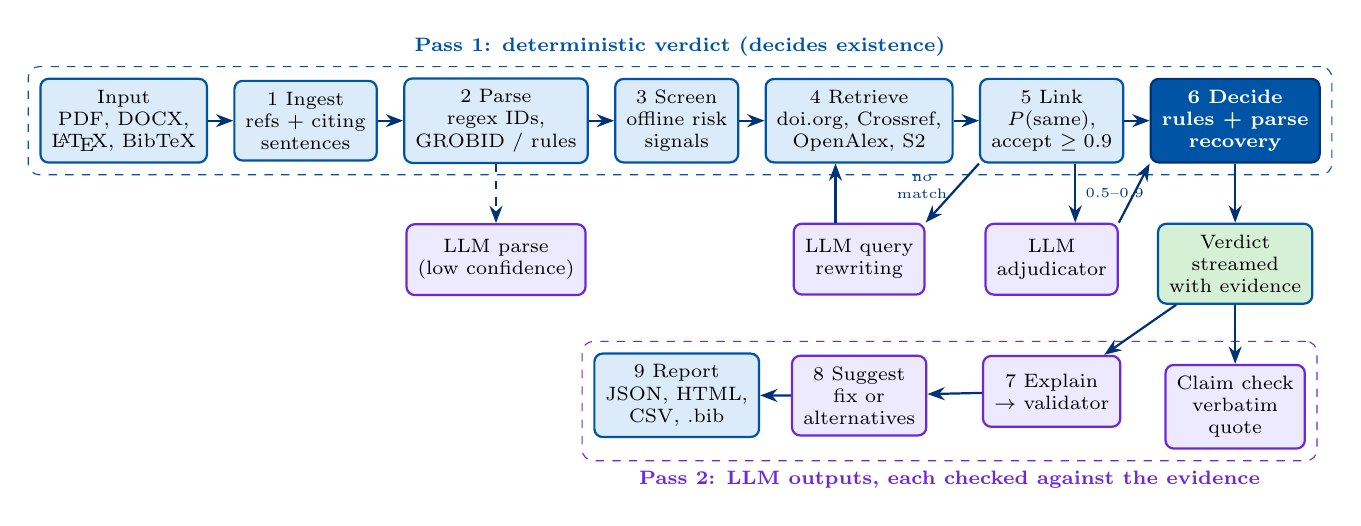
\begin{tikzpicture}[node distance=0.35cm and 0.32cm]
    % row 1: deterministic verdict path
    \node[box, minimum width=1.55cm] (in) {Input\\ PDF, DOCX,\\ \LaTeX, BibTeX};
    \node[box, right=of in, minimum width=1.55cm] (ing) {1 Ingest\\ refs + citing\\ sentences};
    \node[box, right=of ing, minimum width=1.55cm] (par) {2 Parse\\ regex IDs,\\ GROBID / rules};
    \node[box, right=of par, minimum width=1.55cm] (scr) {3 Screen\\ offline risk\\ signals};
    \node[box, right=of scr, minimum width=1.55cm] (ret) {4 Retrieve\\ doi.org, Crossref,\\ OpenAlex, S2};
    \node[box, right=of ret, minimum width=1.55cm] (lnk) {5 Link\\ $P(\text{same})$,\\ accept $\ge 0.9$};
    \node[dbox, right=of lnk, minimum width=1.55cm] (dec) {6 Decide\\ rules + parse\\ recovery};
    % row 2: LLM helpers
    \node[lbox, below=0.75cm of par, minimum width=1.55cm] (lpar) {LLM parse\\ (low confidence)};
    \node[lbox, below=0.75cm of ret, minimum width=1.55cm] (ref) {LLM query\\ rewriting};
    \node[lbox, below=0.75cm of lnk, minimum width=1.55cm] (adj) {LLM\\ adjudicator};
    \node[box, below=0.75cm of dec, minimum width=1.55cm, fill=goodgreen] (ver) {Verdict\\ streamed\\ with evidence};
    % row 3: pass 2
    \node[lbox, below=0.75cm of adj, minimum width=1.55cm] (exp) {7 Explain\\ $\rightarrow$ validator};
    \node[lbox, below=0.75cm of ref, minimum width=1.55cm] (sug) {8 Suggest\\ fix or\\ alternatives};
    \node[box, below=0.75cm of scr, yshift=-1.65cm, minimum width=1.55cm] (rep) {9 Report\\ JSON, HTML,\\ CSV, .bib};
    \node[lbox, below=0.75cm of ver, minimum width=1.55cm] (clm) {Claim check\\ verbatim\\ quote};

    \draw[arr] (in) -- (ing);
    \draw[arr] (ing) -- (par);
    \draw[arr] (par) -- (scr);
    \draw[arr] (scr) -- (ret);
    \draw[arr] (ret) -- (lnk);
    \draw[arr] (lnk) -- (dec);
    \draw[arr, dashed] (par) -- (lpar);
    \draw[arr] (lnk.south west) -- node[lbl, left, pos=0.4] {no\\ match} (ref.north east);
    \draw[arr] ([xshift=-3mm]ref.north) -- ([xshift=-3mm]ret.south);
    \draw[arr] ([xshift=3mm]lnk.south) -- node[lbl, right] {0.5--0.9} ([xshift=3mm]adj.north);
    \draw[arr] (adj.north east) -- (dec.south west);
    \draw[arr] (dec) -- (ver);
    \draw[arr] (ver) -- (exp);
    \draw[arr] (ver) -- (clm);
    \draw[arr] (exp) -- (sug);
    \draw[arr] (sug) -- (rep);

    \begin{scope}[on background layer]
      \node[draw=accentblue, dashed, rounded corners, fit=(in)(dec), inner sep=4pt,
            label={[font=\scriptsize\bfseries, text=accentblue]above:Pass 1: deterministic verdict (decides existence)}] {};
      \node[draw=llmborder, dashed, rounded corners, fit=(rep)(clm), inner sep=4pt,
            label={[font=\scriptsize\bfseries, text=llmborder]below:Pass 2: LLM outputs, each checked against the evidence}] {};
    \end{scope}
  \end{tikzpicture}

  \vspace{2pt}
  \scriptsize Blue: deterministic. Purple: LLM (Groq), output validated before use. Web app,
  REST API and CLI share one engine.
\end{frame}

% =====================================================================
\section{Results}

\begin{frame}{Experimental Results: Fresh Held-Out Split (\texttt{test3})}
  \centering
  \scriptsize
  \renewcommand{\arraystretch}{1.15}
  \begin{tabular}{l ccc cc r}
    \toprule
    & \multicolumn{3}{c}{Fake detection} & \multicolumn{2}{c}{Called fake (\%) $\downarrow$} & LLM \\
    \cmidrule(lr){2-4}\cmidrule(lr){5-6}
    System & P & R & F1 & correct & real & tok./cit. \\
    \midrule
    Offline heuristics only & 1.000 & 0.050 & 0.095 & 0.0 & 0.0 & 0 \\
    DOI lookup only \cite{hallmark} & \na & 0.000 & 0.000 & 0.0 & 11.1 & 0 \\
    \midrule
    LLM-only, \texttt{gpt-oss-20b} & 0.632 & 0.800 & 0.706 & 10.0 & 31.1 & 784 \\
    LLM-only, \texttt{qwen3.8-27b} & 0.506 & 0.700 & 0.587 & \bad{31.7} & \bad{45.6} & 220 \\
    LLM-only, \texttt{gpt-oss-120b} & 0.667 & 0.800 & 0.727 & 13.3 & 26.7 & 671 \\
    \midrule
    \rowcolor{goodgreen}
    CiteGuard, exact matching only & 1.000 & 1.000 & 1.000 & 0.0 & 0.0 & 0 \\
    \rowcolor{goodgreen}
    CiteGuard, deterministic (no LLM) & 1.000 & 1.000 & 1.000 & 0.0 & 0.0 & 0 \\
    \rowcolor{goodgreen}
    CiteGuard, full (Groq LLM) & 1.000 & 1.000 & 1.000 & 0.0 & 0.0 & 241 \\
    \bottomrule
  \end{tabular}
  \vspace{4pt}

  \begin{columns}[T]
    \begin{column}{0.49\textwidth}
      \begin{block}{Finding}
        \scriptsize CiteGuard finds \hl{all 60 fakes} and calls \hl{no real citation fake}. The best
        LLM-only judge calls \bad{13\%} of correct citations fake.
      \end{block}
    \end{column}
    \begin{column}{0.49\textwidth}
      \begin{alertblock}{Honest negative result}
        \scriptsize The LLM changes \hl{no verdict} here, and exact matching is as good: the synthetic
        data is too clean to show their value.
      \end{alertblock}
    \end{column}
  \end{columns}
\end{frame}

\begin{frame}{Experimental Results: LLM-Only Errors, Grounding and Claims}
  \begin{columns}[T]
    \begin{column}{0.52\textwidth}
      \textbf{\textcolor{darkblue}{LLM-only answers on \texttt{test3}}} \scriptsize (exists / fake / unsure)
      \vspace{2pt}

      \scriptsize
      \setlength{\tabcolsep}{3pt}
      \begin{tabular}{l ccc}
        \toprule
        Gold group & \texttt{gpt-oss-20b} & \texttt{qwen3.8-27b} & \texttt{gpt-oss-120b} \\
        \midrule
        Correct (60) & 34 / \bad{6} / 20 & 25 / \bad{19} / 16 & 12 / \bad{8} / 40 \\
        Real w/ errors (30) & 4 / 22 / 4 & 2 / 22 / 6 & 2 / 16 / 12 \\
        Misattributed (20) & 5 / 11 / 4 & 1 / 12 / 7 & 2 / 11 / 7 \\
        Fabricated (40) & 1 / 37 / 2 & 0 / 30 / 10 & 0 / 37 / 3 \\
        \bottomrule
      \end{tabular}
      \vspace{4pt}

      \small They catch fakes mainly because they \hl{distrust what they do not recognise}, and the
      same distrust flags real papers.
      \vspace{4pt}

      \textbf{\textcolor{darkblue}{Earlier held-out splits (first score)}}\\
      \scriptsize Real citations called fake: \texttt{test} 5.6\% $\rightarrow$ \texttt{test2} 1.1\%
      $\rightarrow$ \texttt{test3} \hl{0\%}, fake recall 1.000 throughout.
    \end{column}
    \begin{column}{0.46\textwidth}
      \begin{block}{Grounded explanations}
        \small \hl{19 / 19} LLM explanations passed the evidence validator (1 retry allowed).
      \end{block}
      \begin{block}{Claim-support check (25 papers)}
        \small
        \begin{itemize}
          \item Own conclusion: \hl{25 / 25} supported, \hl{0} false alarms.
          \item Other paper's conclusion: \hl{23 / 25} flagged not supported.
        \end{itemize}
      \end{block}
      \begin{exampleblock}{Self-check}
        \small Our report's 30 references: 28 verified, 2 minor metadata differences, \hl{0 fake}.
      \end{exampleblock}
    \end{column}
  \end{columns}
\end{frame}

% =====================================================================
\section{Discussion}

\begin{frame}{Challenges Faced}
  \begin{columns}[T]
    \begin{column}{0.49\textwidth}
      \begin{block}{Messy reference formats}
        \scriptsize Vancouver names (``Van Tinteren H'', ``Helland \AA''), ``St.\ Petersburg'',
        ALL-CAPS titles, PDF hyphenation marks turned real papers into ``fakes''.\\
        $\Rightarrow$ \hl{Unicode-aware parser + parse-recovery safety net.}
      \end{block}
      \begin{block}{External APIs}
        \scriptsize Crossref / OpenAlex / Semantic Scholar time-outs and rate limits; Groq free tier
        allows 8K tokens per minute.\\
        $\Rightarrow$ \hl{20 s deadline per call, circuit breakers, caching, token limiter.}
      \end{block}
    \end{column}
    \begin{column}{0.49\textwidth}
      \begin{block}{Unreliable LLM output}
        \scriptsize About 1 in 5 strict-JSON calls failed (\texttt{json\_validate\_failed}); one
        headline called a real paper ``fabricated''; one was only a label.\\
        $\Rightarrow$ \hl{Same-model retry, schema checks, evidence validator, template fallback.}
      \end{block}
      \begin{block}{Honest evaluation}
        \scriptsize Synthetic data saturates; fixing errors on test data inflates scores.\\
        $\Rightarrow$ \hl{Each split scored once; a fresh \texttt{test3} for the report.}
      \end{block}
    \end{column}
  \end{columns}
\end{frame}

\begin{frame}{Major Learnings from the Project}
  \begin{enumerate}
    \item \hl{Evidence before generation.} An LLM is a poor oracle for facts it may not know, but a
          good assistant when its output can be checked against evidence.
    \item \hl{False positives are the metric.} Calling a real paper fake costs a user more than
          missing a rare fake, so we report the false-positive rate on correct citations separately.
    \item \hl{``Not found'' $\neq$ ``fake''.} An explicit \emph{Unverifiable} verdict keeps thin
          database coverage from becoming an accusation.
    \item \hl{Structured output still fails.} Strict schemas, validators and fallbacks are needed
          around every LLM call.
    \item \hl{Evaluate like a researcher.} A fresh held-out split and a recorded demo exposed errors the
          development set never showed, and a negative result is still a result.
  \end{enumerate}
\end{frame}

% =====================================================================
\section{Demo}

\begin{frame}{Demo: Web Application}
  \begin{columns}[T]
    \begin{column}{0.49\textwidth}
      \centering
      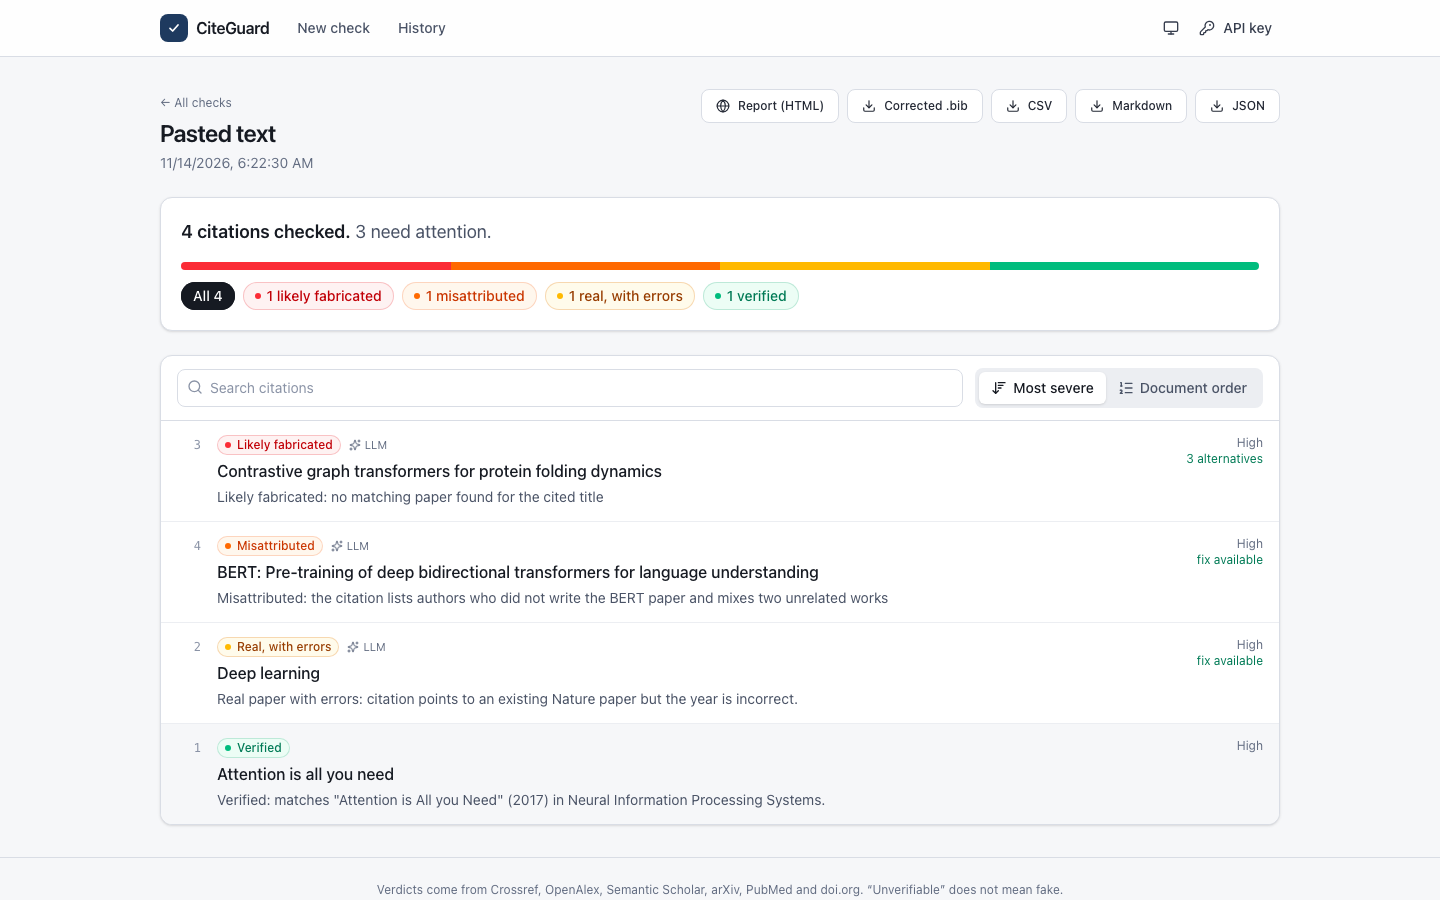
\includegraphics[width=\linewidth]{demo_results.png}\\
      \scriptsize Verdicts for a mixed reference list
    \end{column}
    \begin{column}{0.49\textwidth}
      \centering
      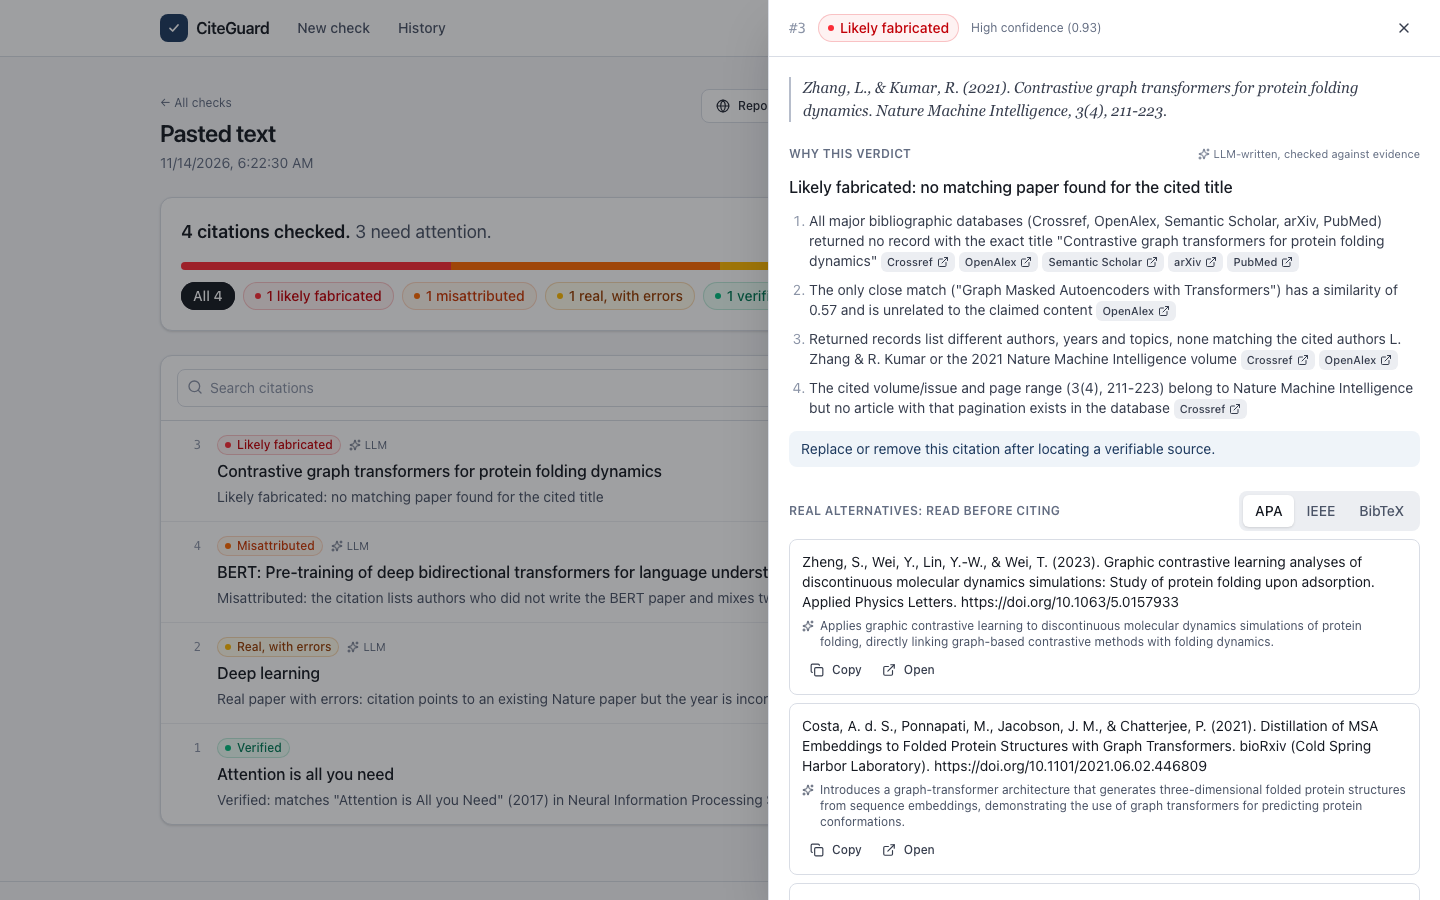
\includegraphics[width=\linewidth]{demo_drawer.png}\\
      \scriptsize Evidence, validated explanation and real alternatives for a fabricated citation
    \end{column}
  \end{columns}
  \vspace{6pt}
  \begin{block}{Run it}
    \scriptsize
    \textbf{Web app:} \texttt{make up} $\rightarrow$ \url{http://localhost:8088} \quad
    \textbf{CLI:} \texttt{citeguard check refs.bib} \quad
    \textbf{REST API:} \texttt{/api/v1/checks} \quad
    \textbf{Video:} \texttt{demo/citeguard\_demo.webm}
  \end{block}
\end{frame}

\begin{frame}{References}
  \scriptsize
  \setbeamertemplate{bibliography item}[text]
  \begin{thebibliography}{99}\setlength{\itemsep}{0pt}
    \bibitem{walters} W.~H.~Walters, E.~I.~Wilder. Fabrication and errors in the bibliographic citations generated by ChatGPT. \emph{Scientific Reports}, 13:14045, 2023. doi:10.1038/s41598-023-41032-5.
    \bibitem{zhao} Z.~Zhao, Y.~Wang, T.~Stuart, M.~De Vaan, P.~Ginsparg, Y.~Yin. LLM hallucinations in the wild: Large-scale evidence from non-existent citations. arXiv:2605.07723, 2026.
    \bibitem{hallmark} K.~Kim, W.~Brendel, P.~Reizinger. HALLMARK: How to diagnose LLM citation verifiers and when to deploy them. arXiv:2607.18360, 2026.
    \bibitem{agrawal} A.~Agrawal, M.~Suzgun, L.~Mackey, A.~T.~Kalai. Do language models know when they're hallucinating references? \emph{Findings of EACL}, 912--928, 2024.
    \bibitem{citecheck} K.~Khajavi, S.~Sadeghi, R.~Adhikari, A.~Tessier. CiteCheck: Retrieval-grounded detection of LLM citation hallucinations in scientific text. arXiv:2605.27700, 2026.
    \bibitem{citetracer} M.~Li, Z.~Lin, S.~Ma. Source or it didn't happen: A multi-agent framework for citation hallucination detection. arXiv:2605.08583, 2026.
    \bibitem{grobid} P.~Lopez. GROBID: Combining automatic bibliographic data recognition and term extraction for scholarship publications. \emph{ECDL}, LNCS 5714, 473--474, 2009.
    \bibitem{fellegi} I.~P.~Fellegi, A.~B.~Sunter. A theory for record linkage. \emph{JASA}, 64(328):1183--1210, 1969.
    \bibitem{gptoss} OpenAI. gpt-oss-120b \& gpt-oss-20b model card. arXiv:2508.10925, 2025.
  \end{thebibliography}
  \vspace{2pt}
  \tiny All references were verified with CiteGuard itself. Full list in the project report (\texttt{paper/main.pdf}).
\end{frame}

\begin{frame}[plain]
  \centering
  \vspace{0.5cm}
  
\begin{tikzpicture}
    \node[fill=accentblue, text=white, rounded corners=6pt, minimum width=0.6\paperwidth,
          minimum height=1.5cm, font=\Huge\bfseries] {Thank You};
  \end{tikzpicture}
  \vspace{0.3cm}

  {\Large\textcolor{darkblue}{Questions \& Discussion}}\\[0.5cm]
  \begin{columns}[c]
    \begin{column}{0.62\textwidth}
      \small
      \textbf{\textcolor{darkblue}{GitHub:}}
      \url{https://github.com/mjgandhi2305/ILLM_FinalProject_Citeguard}\\[4pt]
      \textbf{\textcolor{darkblue}{Hugging Face:}} none (no trained weights; uses Groq-hosted
      \texttt{gpt-oss} models)\\[4pt]
      \textbf{\textcolor{darkblue}{Demo:}} web app, CLI, REST API, recorded video in \texttt{demo/}\\[4pt]
      \textbf{\textcolor{darkblue}{Report:}} \texttt{paper/main.pdf}\\[8pt]
      \scriptsize Miten Gandhi (U23AI017) $\cdot$ Harshil Andhariya (U23AI021) $\cdot$
      Vatsal Bateriwala (U23AI030) $\cdot$ Aksh Dharodiya (U23AI031)
    \end{column}
    \begin{column}{0.28\textwidth}
      \centering
      
\includegraphics[width=0.85\linewidth]{github_qr.png}\\
      \scriptsize Scan for the repository
    \end{column}
  \end{columns}
\end{frame}

\end{document}
